\documentclass{scrreprt}

\usepackage{lmodern}
\usepackage[utf8x]{inputenc}
\usepackage[ngerman]{babel}
\usepackage{microtype}
\usepackage{enumitem}

\usepackage{xcolor}
\usepackage{longtable}
\usepackage{todonotes} % not found!?


\usepackage{vmargin}
\setpapersize{A4} % besser oben?
\setmarginsrb{3cm}{1.5cm}{3cm}{1cm}{6mm}{6mm}{5mm}{15mm}

% Tiefe d. Inh. VZ
\setcounter{secnumdepth}{3}
\setcounter{tocdepth}{3} 




\usepackage{graphicx}
\usepackage{svg}
\usepackage{hyperref}


\begin{document}

	\title{	
	%
		Pflichtenheft\\~\\~\\
		\Huge{KNOT$^3$}\\~\\
		\Large (\href{http://pp.info.uni-karlsruhe.de/lehre/WS201314/pse/}{Praxis der Softwareentwicklung am KIT}: Echtzeit-Computergrafik in der Spieleentwicklung \\am \href{http://cg.ibds.kit.edu/index.php}{Lehrstuhl für Computergrafik})
	%
	}
	
	\author{
	%
		Tobias Schulz, Maximilian Reuter, Pascal Knodel,\\
	 	Gerd Augsburg, Christina Erler, Daniel Warzel
	%
	} 
	 
	\date{\today}
	
	\maketitle
	% %TODO: Vorlage mit:
	% Titel
	% (KIT-/Knot³)Logo (wenn möglich)
	% Felder für Veranstaltung, 
	% PSE-Teilnehmer, 
	% Betreuer, 
	% Versionsnummer, 
	% Erstes Datum und das der letzten Aktualisierung ...

	\tableofcontents
<<<<<<< HEAD

	\chapter{Einleitung}
Nach Pflichtenheft und Entwurf stand nun die Implementierung auf dem Plan.
Auf den folgenden Seiten beschreiben wir, wie das vonstattenging, welche Änderungen wir vornehmen mussten und auf welche Probleme wir gestoßen sind.
Durch die vielfältigen Möglichkeiten, die ein frei veränderbarer Knoten bietet, entstand eine hoch komplexe Interaktionsvielfalt,
von der manche Bereiche im Entwurf nicht ausreichend Beachtung fanden, bzw. finden konnte.
Dadurch sind einige Änderungen zum ursprünglichen Entwurf notwendig geworden, die sich aber vor allem auf Erweiterungen bezieht.
Dennoch hat sich unser Entwurf als gut erwiesen, da alle Änderungen ohne Umbau der grundlegenden Strukturen integriert werden konnten.

=======
    % !TeX encoding = UTF-8
%
% Einführung
%


\chapter{Einführung}
% \label{Einführung}
Bei Knot³ handelt es sich um ein innovatives Spiel bei dem man Knoten im Dreidimensionalem Raum entweder frei modifizieren, oder nach Vorgabe auf Zeit ineinander überführen kann.
Die Idee und das Konzept zu diesem Spiel stammt von der Hochschule für Gestaltung in Karlsruhe und wird im Rahmen der Praxis der Softwareentwicklung von Studenten des Karlsruher Instituts für Technologie umgesetzt.


% \section{Interessen} Ist eigentlich gleich mit Zielbestimmung
% Gute Noten!


\section{Konzepte}
Das Konzept des Spieles ist in die Kategorie der Sandbox-Spiele einzuordnen. Es wird nicht wie in klassischen Spielen ein Ziel vorgegeben und verschiedene Wege gegeben dies zu erreichen, sondern es wird dem Spieler überlassen, was er machen will. Dabei bietet man ihm viele Möglichkeiten schöpferisch tätig zu sein. Die Herausforderung und die Motivation entsteht dadurch, dass es kein 3D-Modellierer ist. Man ist ist gezwungen zu abstrahieren, sich Tricks auszudenken um bestimmte Wirkungen zu erzielen und sein selbst gestecktes Ziel zu erreichen. Dabei geht der kreative Prozess schon bei der Auswahl des Motivs los, manche lassen sich besser durch Kanten darstellen als andere.
Genauso gut kann man aber auch Herausforderungen für andere Erstellen. Komplizierte Transformationen, die sich nur schwer nachbauen lassen oder gewaltige Bauten die durch ihre schiere Größe beeindrucken. Und natürlich kann man auch die von anderen Nutzern erstellten Herausforderungen bestreiten und dem Ersteller zeigen, dass sein komplizierter Knoten nicht so schwer zu durchschauen ist wie er ursprünglich dachte.
Einzig die Vorstellungskraft des Spielers limitiert die Möglichkeiten der Anwendung.

\section{Vorstellungen}
Wir erhoffen, dass die Spieler sich übers Internet austauschen und sich gegenseitig zu immer neuen Ideen anregen, Bilder ihrer schönsten Kreationen zeigen und ihre besten Herausforderungen verteilen. In Zukunft wird es viele Nachbauten von berühmten Gebäuden, wie z.B. dem Eiffelturm oder Brandenburger Tor geben, genauso wie abstrakte Gebilde, die die verschiedensten Wirkungen erzielen. Es wird wie bei anderen Sandbox-Spielen Fan-Seiten geben die die Bilder speichern Kategorisieren und auch die dazugehörigen Knotendateien in ihrem Austauschformat bereitstellen. Es wird Kunstprojekte geben, die dieses Programm nutzen um dreidimensionale Gebilde zu erstellen, da es erheblich leichter als ein 3D-Modellierer zu bedienen ist und durch sein offenes Austauschformat leicht in viele andere Formate umgewandelt werden kann, z.B. für den 3D-Druck. Genauso wird es aber auch Spieler geben, die das Programm dazu nutzen ihre räumlich Vorstellung zu stärken zur Entspannung oder als Konzentrationsübung.
Durch seine Freiheit in der Verwendung wird Knot³ darüber hinaus auch noch in Gebieten Verwendung finden die selbst wir uns noch nicht vorstellen können.

>>>>>>> 3d3f9be4e073c7bc062e579dcae267d6637baf3e
	\chapter{Zielbestimmung}

Das Spiel versetzt einen einzelnen Spieler in die Lage Knoten im dreidimensionalen Raum zu erstellen und zu modifizieren. Zwischen den Kanten der Knoten besteht die Möglichkeit Flächen einzusetzen und diese zu texturieren. Zudem wird dem Spieler erlaubt sich in verschiedenen Herausforderungen mit anderen Spielern zu messen.\\


\section{Musskriterien}

\begin{itemize}

	\item Spielmodus 1 Freies Erstellen
	
	\item Spielmodus 2 Challenges
	
	\item Knotenübergänge müssen eindeutig erkennbar sein.
	
	\item Darstellung mit passenden 3D-Modellen an Übergängen.
	
	\item Selektion und Modifkation von Kantenzügen.
	
	\item Übergehen unmöglicher Zustände, wenn möglich.
	
	\item Highscores: Heuristik zur Komplexität / Eindeutigkeit.
	
	\item einfaches Datenaustauschformat für die Levels
	
	\item mindestens zehn eindeutige Level mit steigendem Schwierigkeitsgrad.
	
	\item intuitive Steuerung
	
	\item sinnvolles Undo
	
	\item gute automatische Kameraführung
	
	\item Sound soll unterstützen
	
	\item Tutorials sollen unterstützen
	
	\item  Einfaches Speicherformat das lokal Austauschbar ist
	
\end{itemize}

\section{Kannkriterien}


\begin{itemize}
\item  Shadereffekte

\item Online-Austausch der Leveldaten

\item  3D-Drucker kompatible Ausgabe der Leveldaten
\end{itemize}

	\chapter{Produkteinsatz}

Das Spiel soll Spieler mit Vorliebe für das Gestalten im dreidimensionalem Raum ansprechen sowie auch Spieler die gerne ihre Fähigkeiten im Vorstellen von Räumlichen Sachverhalten mit anderen vergleichen und messen wollen.

\section{Anwendungsbereiche}


\begin{itemize}

	\item Unterhaltungssoftware im Heimanwendungsbereich. 
	
	\item Ein Werkzeug für Künstler zur Modellierung von 3D-Knoten, z.B. als Minikunstwerke, geeignet für den 3D-Druck.
	
	\item Ein Gedächtnis-/Knobelspiel zum Training der
	geistigen Fähigkeiten.
	
	
	
\end{itemize}

\section{Zielgruppen}

Da das Spiel allein von räumlichem Vorstellungsvermögen abhängt kann prinzipiell jeder, der die Bedienung mit Maus und Tastatur versteht es spielen, vorausgesetzt er versteht Englisch.
\\
Das Spiel richtet sich jedoch besonders an Leute die Spaß an kreativem Erstellen von 3D-Knoten haben, bzw. ihr Räumliches Vorstellungsvermögen im Challenge-modus unter Beweis stellen wollen.






	\chapter{Produktumgebung}



\section{Hardware}

\begin{itemize}
\item DirectX 9c-kompatibele Grafikkarte (mindestens Shader Model 3)
\end{itemize}




\section{Software}

\begin{itemize} 
\item Windows XP, Vista, 7, 8 oder 8.1
\begin{itemize}
\item Microsoft .NET Framework 4.5 
\item XNA 4.0
\end{itemize}
\item Linux/Unix
\begin{itemize}
\item Mono 3.0 oder neuer
\item Monogame 3.0.1 oder neuer
\item OpenTK 1.0
\end{itemize}
\end{itemize}



	\chapter{Funktionale Anforderungen}


\begin{description}[itemsep=13pt,parsep=13pt]

\item[/FA10/]
	\begin{description}
	\item[Geschäftsprozess:] 
	\item[Ziel:] 
	\item[Kategorie:] 
	\item[Vorbedingung:] 
	\item[Nachbedingung (Erfolg):]
	\item[Nachbedingung (Fehlschlag):]
		\begin{itemize}
			\item 			
		\end{itemize}
	\item[Akteure:]
	\item[Auslösendes Ereignis:] 
	\item[Beschreibung:] 	
	\end{description}	
		
		

	\chapter{Produktdaten}

\renewcommand{\theenumi}{/PPD\_\arabic{enumi}0/}
\renewcommand{\labelenumi}{\theenumi}

\section{Persistente Daten}

\begin{enumerate}

\item Nutzerprofile speichern Informationen zum Spieler dauerhaft. 

  \begin{itemize}
     \item Nickname
  \end{itemize}

\item Eine Spielestatistik bietet dem aktuellen Spieler eine Übersicht über gebaute Knoten und absolvierte Challenges.

  \begin{itemize}
     \item Spielzeit
     \item Errungenschaften
     \item Bestandene Challenges
     \item Übersicht der Creatives
  \end{itemize}

\item Standard-Spracheinstellungen sind verfügbar

  \begin{itemize}
     \item Deutsche Sprache
     \item Englische Sprache
  \end{itemize}
  
%\item Neue Sprachpakete für die Internationalisierung sind integrierbar.

\item In der Offline-Bestenliste für Challenges wird der Spielername und die Zeit gespeichert.
\item 10-Challenges sind bei jedem Knot³-Spielpaket enthalten.

  \begin{itemize}
     \item Levelname
     \item Empfehlung (Anfänger oder Fortgeschrittene)
  \end{itemize}

\item Standard-Grafikeinstellungen werden beim ersten Spielstart gespeichert. Vom Spieler angepasste Grafikeinstellungen sind auch beim nächsten Start weiterhin aktiv.

\item Weitere Einstellungen

  \begin{itemize}
     \item Sprache
     \item Effekte
     \item (Hintergrund-)Musik
  \end{itemize}

\item Voreingestellte Standard-Steuerungseinstellungen.
\item {\color{red}Spielstände des 2. Modus (Spielstandname, Spieler, Spielzeit, ...) können aus einer eigenen Übersicht ausgewählt und geladen werden.}
\item Die Erfolge und lokale Bestenliste. Für jede Challenge ist eine Bestenliste anzulegen.
\item Die bei der  Entwicklung entstehenden Dokumentationen.
\item Grafiken welche Teil der Benutzeroberfläche sind.
%\item Die Dokumentation des Spiels für den Spielers ist im Hauptmenü abrufbar.
\item Die Online-Bestenliste.

  \begin{itemize}
     \item Spielername
     \item Datum
     \item Erreichte Punkte
     \item Spieldauer
  \end{itemize}
  
\item Die Knot³-Homepage.
\item Die Webseite der Online-Bestenliste.
\item Die Support-Webseite.
\item Informationen zur Erreichbarkeit Webseiten (URLs).
\item Der eine Knoten im Creative(-Mode) und die zwei Knoten im Challenge(-Mode).

  \begin{itemize}
     \item Knoten (im Austauschformat)
     \item Kantenfarben
     \item Texturierung
  \end{itemize}
  
\item Knoten bei Spielständen des 1. Modus werden in einem Format welches 3D-Drucker verstehen gespeichert.
\item Soundeffekt-Dateien, welche Geräusche von Effekten enthalten.
\item Dateien für die Musikstücke, welche als Hintergrundmusik abgespielt werden.



\end{enumerate}

~\\

\renewcommand{\theenumi}{/GPD\_\arabic{enumi}0/}
\renewcommand{\labelenumi}{\theenumi}

\section{Generierbare Daten}


\begin{enumerate}

\item Der Schwierigkeitsgrad muss nicht gespeichert werden, da er dynamisch aus der Knotenstruktur berechnet wird.
\item Die Knoten-Komplexität wird dynamisch berechnet und muss nicht gespeichert werden.

\end{enumerate}

	\chapter{Nichtfunktionale Anforderungen}

\begin{tabular}{|p{0.125\textwidth}|p{0.875\textwidth}|}
\hline 
\textbackslash NF10  \textbackslash & Transformierung des Knotes muss durch die Maus möglich sein\\ % Funktionaler Anteil? % Bedienung mit PC-Standardperipherie muss möglich sein %
\hline 
\textbackslash NF20  \textbackslash & Im manuellen und zentrierten Kamera-Modus muss die Kamera mit Hilfe der Maus oder Tastatur navigierbar sein (Drehen, Zoomen und Bewegen)\\ % Funktionaler Anteil? %
\hline 
\textbackslash NF30  \textbackslash & Das Spiel sollte unter normalen Grafikeinstellungen immer mindestens eine Bildwiederholungsraten von 30 Bilder pro Sekunde haben\\ 
\hline 
\textbackslash NF40  \textbackslash & Grafische Gestaltung der Knoten soll die Übersicht des Spielers nicht einschränken oder verschlechtern\\ 
\hline 
\textbackslash NF50  \textbackslash & Soll bis auf die Installation von .NET ohne Zusätze lauffähig sein.\\ 
\hline 
\textbackslash NF60  \textbackslash & Übersichtliche Menüführung, u.A. durch den Einsatz von Alternativen zur Navigation über aufklappbare Listen.\\ % Funktionaler Anteil? %
\hline 
\textbackslash NF70  \textbackslash & Intuitive Spielsteuerung, welche auch durch Ausprobieren schnell erlernbar ist.\\ 
\hline 
\textbackslash NF80  \textbackslash & Erweiterbarkeit durch Einbindung von Internationalisierungen.\\ % !!! %
\hline 
\textbackslash NF90  \textbackslash & Einstellen kontrastreicher Farben für Menschen mit "eingeschränkter Sehstärke".\\ 
\hline
\textbackslash NF100  \textbackslash & Betrügereien bei den Highscores sollen automatisch erkannt/ersichtlich werden.\\ 
\hline 
\textbackslash NF110  \textbackslash & Starten- und anschließendes Beenden muss in weniger als 45 Sekunden möglich sein.\\ % !!! Besserer Wert? %
\hline
\textbackslash NF120  \textbackslash & Speichern von Spielständen darf den Dialog mit dem Spieler nicht wesentlich verzögern.\\ % !!! Besserer Wert? %
\hline
\end{tabular} 

	\chapter{Globale Testfälle}

\renewcommand{\theenumi}{/T\_\arabic{enumi}0/}
\renewcommand{\labelenumi}{\theenumi}

\section{Funktionstests}

\begin{enumerate}
\item Die Grafikauflösung wird im Einstellungsmenü verändert.\\
	 	\textit{Erwartet:} Das Spiel verwendet die gewünschte Auflösung, sofern diese vom System unterstützt wird. Falls nicht, wird eine Fehlermeldung eingeblendet, die darauf hinweist, dass diese Einstellung nicht möglich ist. Die Auflösung wird in diesem Fall nicht geändert.
	 	
\item Die Lautstärke der Musik und Toneffekte wird im Einstellungsmenü angepasst. \\  
\textit{Erwartet:} Bei erhöhter Lautstärke wird die Musik oder die Toneffekte lauter abgespielt als bei niedrigeren Einstellungen. Die Soundeffekte oder Musik werden nicht abgespielt wenn die Lautstärke auf den Wert 0 gestellt wurde. Falls nur die Musik auf dem Wert 0 steht, wird nur die Musik nicht abgespielt, aber die Toneffekte werden mit ihrer Lautstärke weiterhin ausgegeben.
\item Beenden des Spiels über das Hauptmenü.\\
\textit{Erwartet:} Das Spiel schließt sich vollständig, d.h. alle laufenden Prozesse des Spieles werden beendet und der Speicher wird freigeben.
\item Verlassen eines aktiven Spiels über das Pause-Menü.\\
\textit{Erwartet:} Nach dem Klicken auf den Beenden-Button, des Pause-Menüs erscheint das Hauptmenü.
\item Transformieren des Knotens, sowohl im Challenge-Modus als auch im Creative-Modus.\\
\textit{Erwartet:} Falls die Transformation gültig ist, wird die Kante entsprechend transformiert. Dies funktioniert, sowohl im Challenge-Modus als auch im Creative-Modus.
\item Kamerapostion verändern (bewegen, drehen und zoomen), sowohl im Challenge-Modus als auch im Creative-Modus.\\
\textit{Erwartet:} Die Kameraposition verändert sich wie gewünscht in die vorgegebene Richtung. Dies funktioniert, sowohl im Challenge-Modus als auch im Creative-Modus.
\item Erfolgreiches Beenden einer Challenge. \\
\textit{Erwartet:} Die Zeit wird gestoppt und der Abschlussbildschirm wird eingeblendet. Falls die Zeit für die Bestenliste ausgereicht hat, wird diese direkt eingetragen.
\item Speicherung eines Knotens den man im Creative-Modus erstellt hat und späteres Laden.\\
\textit{Erwartet:} Ein Knoten wird in einer Datei im Austauschformat gespeichert. Wenn diese Datei geladen wird erhält man den vorher abgespeicherten Knoten zurück.
\item Installation des Spiels auf Windows Zielsystemen
\item Restlose Deinstallation des Spiels von Windows Zielsystemen.

\end{enumerate}


\section{Robustheitstests}


\begin{enumerate}[resume]
\item Rückgängig machen beliebig vieler Knoten-Transformationen. 
\item Wiederholen von rückgängig gemachten Schritten.
\item Wahllose Eingaben führen nicht zum Absturz.
\end{enumerate}




	%\chapter{Entwicklung}

\section{Software}

\begin{itemize}


\item GitHub-Client
\item LateX (unterstützt durch Incscape und perl)
\item Visual Studio 2013
\item C-Sharp
\item ...

\end{itemize} % ToDo: ich glaub hier hab ich mich vertan, aber nochmal schauen ... nein, habe mich doch nicht vertan, war korrekt, rein!
	\chapter{Systemmodelle}


\section{Interaktionsverlauf}

	\begin{longtable}{|p{0.25\textwidth}|p{0.75\textwidth}|}
    \hline
    main menu & Das ist die erste Ansicht, die der Nutzer bekommt. Von hier aus erreicht er alle Bereiche des Programms.\\
    \hline
    creative & Von hier aus startet der Nutzer ein neues Spiel, mit einem einfachem Standardknoten, lädt einen Speicherstand oder startet das erstellen von neuen Herausforderungen (challenges).\\
    \hline
    challenge & Eine Übersicht, der vorhandenen Herausforderungen. Der Nutzer kann nach verschieden Kriterien suchen und sortieren lassen und in einer Vorschau weitere Informationen betrachten.\\
    \hline
    settings & Einstellungen an Grafik, Ton und Steuerung. Außerdem kann die persönliche Farbpalette angepasst werden.\\
    \hline
    credits & Zeigt Infos über die Mitwirkenden an dem Programm und über das Programm selber.\\
    \hline
    
   \end{longtable}
   
   ~\\
    
	\begin{figure}[h]
		\centering
	 	\includesvg[width = 0.95\textwidth]{menu}
	 	\caption{Hauptmenüeinträge}
	\end{figure}
	
	\clearpage
	~\\
	
	Im Spiel kann der Nutzer auch die {\color{red} Einstellungen} erreichen. Die Menüeinträge in den unterschiedlichen Spielmodi können variieren.
<<<<<<< HEAD
		
	\begin{longtable}{|p{0.25\textwidth}|p{0.75\textwidth}|}
	
	\hline
	settings & Genau wie aus dem Hauptmenü.\\
	\hline
	save & Speichert den aktuellen Spielstand.\\
	\hline
	quit & Beendet das laufende Spiel. \\
	\hline
	render options & Bietet dem Nutzer verschiedene Möglichkeiten seinen Knoten zu rendern und zu exportieren.\\
	\hline
	
	\end{longtable}
	
	\begin{figure}[!ht]
		  \centering
		  \includesvg[width = \textwidth]{ingamemenu}
		  \caption{Menü f. Einstellungen während des Spiels.}
	\end{figure}
=======
\begin{longtable}{|p{0.25\textwidth}|p{0.75\textwidth}|}

	settings & Genau wie aus dem Hauptmenü.
    \hline
	save & Speichert den aktuellen Spielstand.
    \hline
	quit & Beendet das laufende Spiel.
    \hline
	render options & Bietet dem Nutzer verschiedene Möglichkeiten seinen Knoten zu rendern und zu exportieren.
\end{longtable}

>>>>>>> 3d3f9be4e073c7bc062e579dcae267d6637baf3e
	
\clearpage


\section{Benutzerinteraktionsmodelle}

	\begin{figure}[ht]
		  \centering
		  \includesvg[width = 0.9\textwidth]{Auswahl}
	\end{figure}
	
\clearpage

\subsection{Spielzüge}

~\\
...

\subsubsection{Beispiele gültiger Züge}

~\\
...

\subsubsection{Beispiele ungültiger Züge}

	\begin{figure}[htb]
	  \centering
	  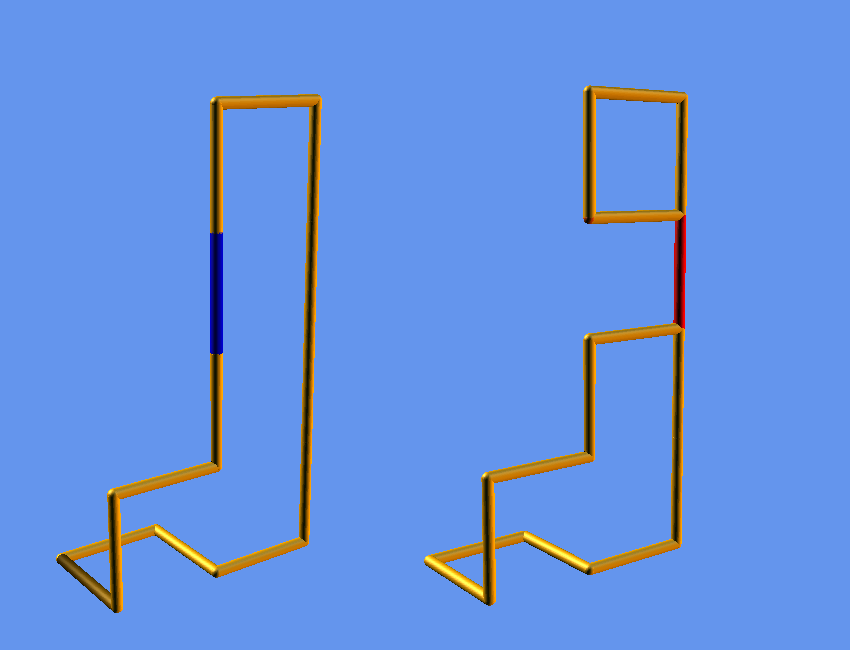
\includegraphics[width = \textwidth]{Systemmodelle/Ungueltiger_Zug.png}
	  \caption{Parallele Kantenvereinigung}
	  \label{fig:zug1}
	\end{figure}

Der Knoten auf der linken Seite \ref{fig:zug1} beschreibt eine gültige Spielsituation. Der Spieler wählt eine Kante (blaue Hervorhebung) aus, um einen weiteren Zug vorzunehmen.
Einem Spieler ist es nicht möglich, zwei parallele Kanten (hier: die Blaue und die Rote) zu einer Kante zu vereinen. Der Knoten soll immer aus einem geschlossenen Kreis von Kanten bestehen. Der Knoten auf der rechten Seite \ref{fig:zug1} ist daher eine ungültige Spielsituation.

\clearpage

	\begin{figure}[htb]
	  \centering
	  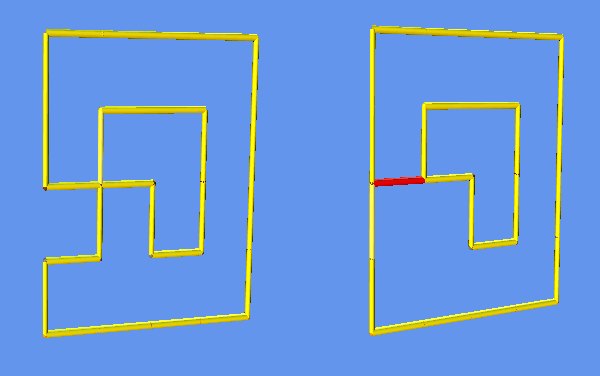
\includegraphics[width = \textwidth]{Systemmodelle/Ungueltiger_Zug2.png}
	  \caption{{\color{red}Änderung der Kantenzuordnung}}
	  \label{fig:zug2}
	\end{figure}
	
Auf der 

\clearpage

\section{Grafische Bedienuns-Oberflächen}

	\begin{figure}[ht]
	  \centering
	  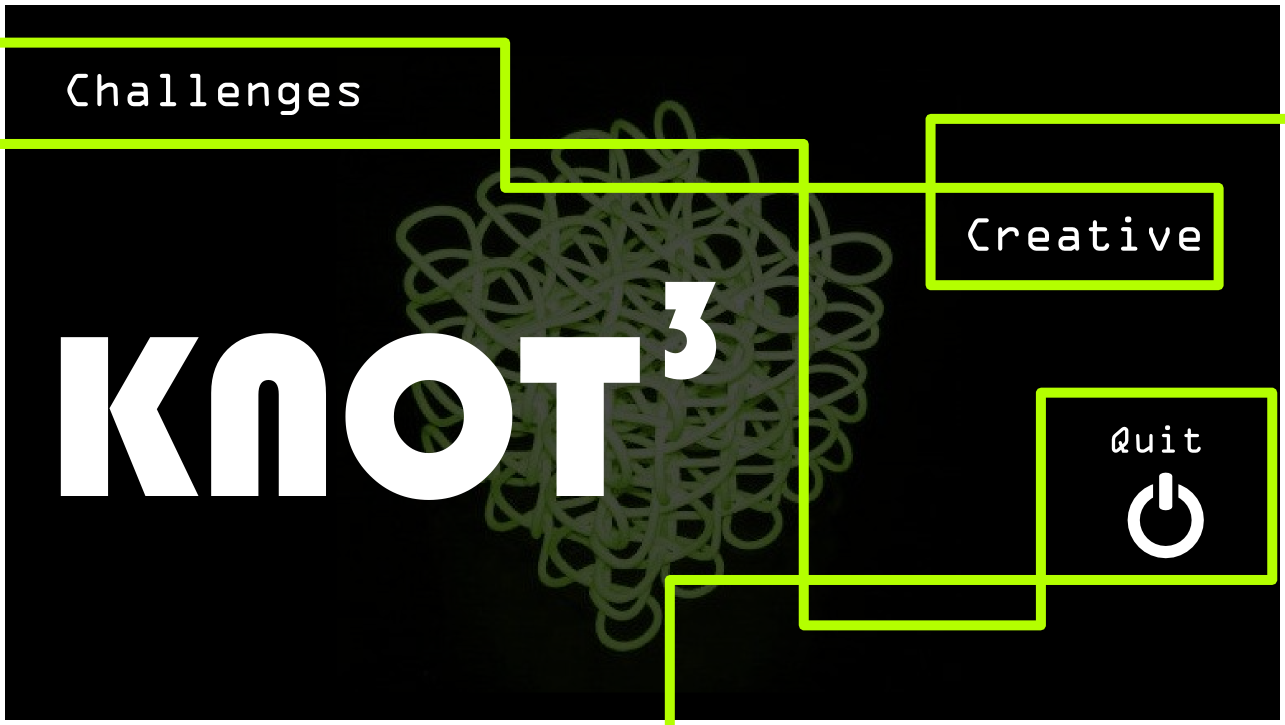
\includegraphics[width = 0.95\textwidth]{Systemmodelle/01_Knot3-mainscreen.png}
	  \caption{Hauptmenü}
	\end{figure}

	\begin{figure}[ht]
	  \centering
	  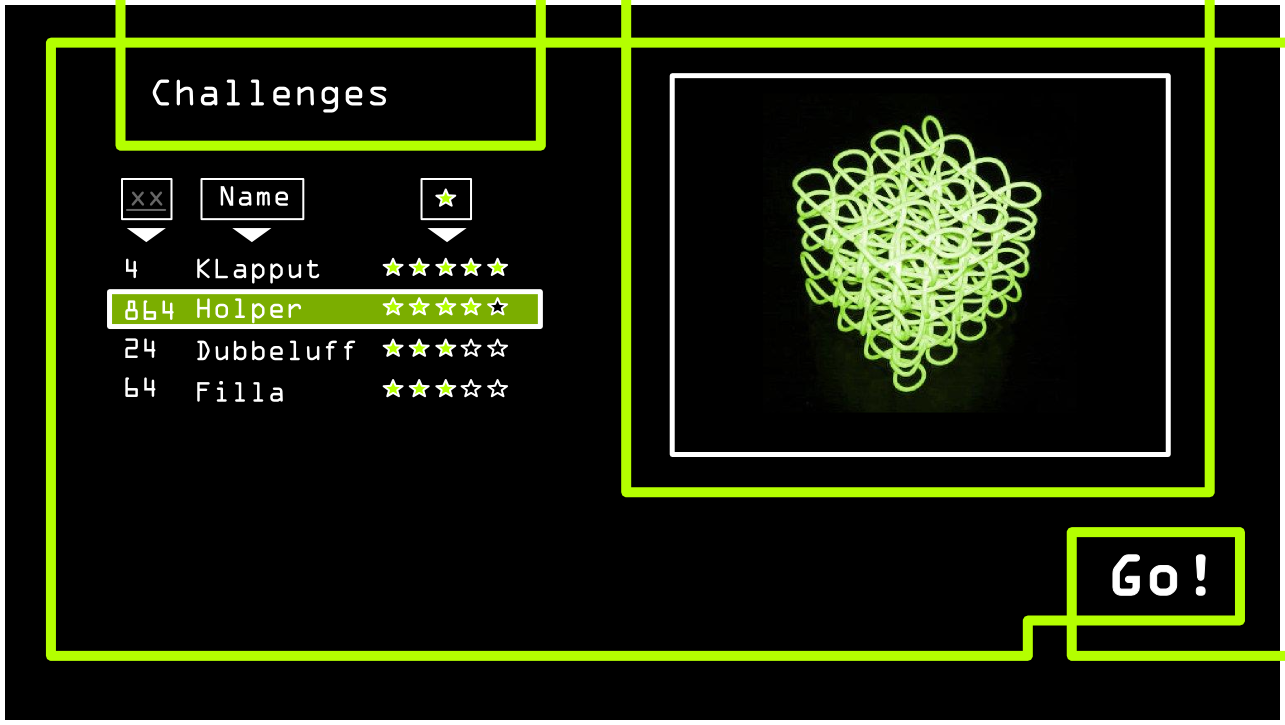
\includegraphics[width = 0.95\textwidth]{Systemmodelle/04_Knot3-select-Challenge.png}
	  \caption{Menü für Herausforderungen, mit Ausschnitt der Bestenliste}
	\end{figure}
	
	\begin{figure}[ht]
	  \centering
	  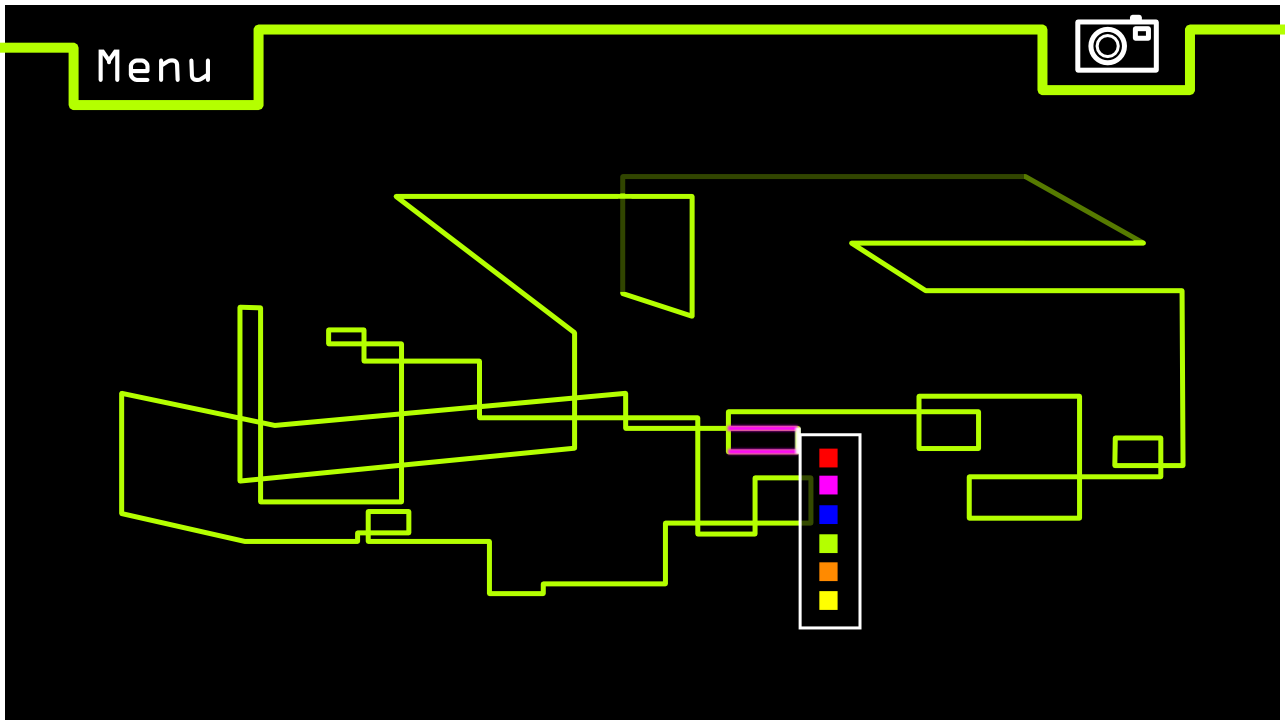
\includegraphics[width = 0.95\textwidth]{Systemmodelle/05_Knot3-Colour-select.png}
	  \caption{Creative: Kantenfärben}
	\end{figure}
	
	\begin{figure}[ht]
	  \centering
	  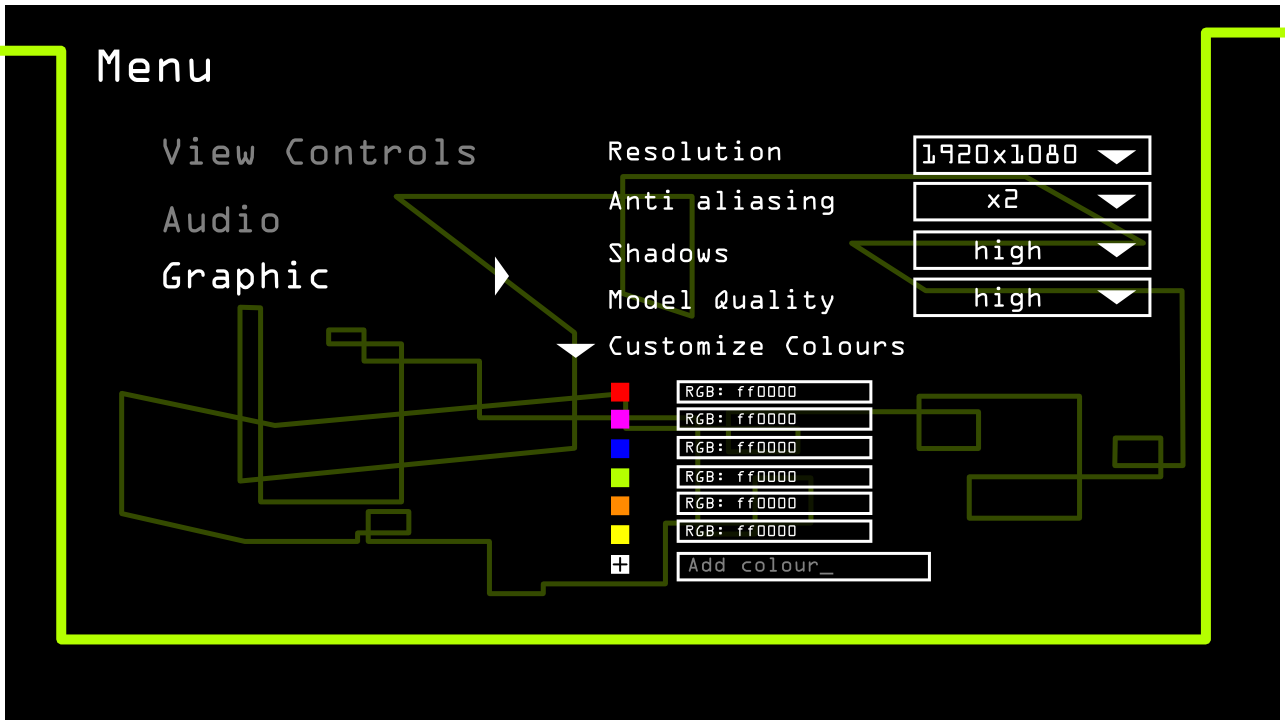
\includegraphics[width = 0.95\textwidth]{Systemmodelle/08_Knot3-menu-graphics.png}
	  \caption{Menü f. Grafikeinstellungen}
	\end{figure}

	
\clearpage
	
\section{Szenarien}
\begin{itemize}	
\item Der Spieler startet das Spiel und gelangt zum Hauptmenü. Dort wählt er den "creative" Modus und im darauf folgendem Menü das Erstellen eines neuen Knotens. Er gelangt in den Editor und beginnt dort den Knoten zu transformieren. Nach einigen transformationen öffnet er das Menü und speichert den Knoten. Danach fährt er mit der transformation fort. Zwischendurch ist er mit einigen Transformationsschritten unzufrieden und macht sie mir "undo" rückgängig. Nach einigen weiteren transformationen ruft er wieder das Menü auf, speichert und beendet daraufhin den Editor mit einem klick auf den Menüeintrag "quit". Daraufhin landet er wieder im Hauptmenü. Dort beendet er das Spiel.

\item Der Spieler startet das Spiel und gelangt zum Hauptmenü. Dort wählt er den "creative" Modus und danch "load" um einen alten Speicherstand zu laden. In der Auswahlliste wählt er den gewünschten Knoten aus und lädt diesen. Er landet im Editor. Dort betrachtet er Knoten ein Zeitlang von allen Seiten, indem er mit Tastatur und Maus die Kamera um den Knoten herum bewegt und beendet danach wieder den Editor.

\item  Der Spieler startet das Spiel und gelangt zum Hauptmenü. Dort wählt er den "challenge" Modus. Er sieht eine Liste mit allen verfügbaren Herausforderungen und einige Informationen zu diesen, dazu gehören die aktuellen Bestzeiten. Er sucht sich eine Herausforderung aus und Startet sie. Er landet im Editor mit einer zusätzlichen Ansicht für den Zielknoten. Er betrachtet diesen ausgiebig und beginnt danach mit der Transformation des vorgegebenen Knotens. Zum Zeitpunkt der ersten Transformation beginnt die Zeit zu laufen. Nach einigen Transformation stimmen die Knoten überein und die Zeit stoppt automatisch. Der Spieler war schnell und darf seinen Namen in die Bestenliste eintragen. Danach hat er die Möglichkeit die Herausforderung zu bewerten. Er gibt der Herausforderung eine gute Bewertung und landet danach wieder im Hauptmenü. Dort beendet er das Spiel.

\item Der Spieler startet das Spiel und gelangt zum Hauptmenü. Dort wählt er den "creative" Modus. Er möchte eine neue Herausforderung erstellen und wählt daher "new challenge". Danach wählt er zwei Knoten aus seinen Speicherständen aus. Einen für den Startknoten, einen als Zielknoten. Weiter unten gibt er der Herausforderung einen Namen und Speichert sie ab. Danach gelangt er in den Editor um als erster eine Zeit vorzulegen und die Herausfforderung zu bestreiten. Der Spieler beendet dei Herausforderung aber ohne sie abzuschließen. Er kann die Herausforderung noch bewerten und landet dann wieder im Hauptmenü. Dort beendet er das Spiel.
\end{itemize}

~\\
...

	\begin{figure}[ht]
	  \centering
	  \includesvg[svgpath=Systemmodelle/, width = \textwidth]{inGame}
	  \caption{Interaktionen während eines Spiels (allgemein)}
	\end{figure}

%	\begin{figure}[ht]
%	  \centering
%	  \includesvg[width = \textwidth]{Anwendungsfall}
%	  %\caption{...}
%	\end{figure}


	\chapter{Glossar}

\begin{tabular}{|p{0.25\textwidth}|p{0.75\textwidth}|}
\hline 
\ Knot~$^3$ & Spielkonzept und Spiel-Name (engl. für Knoten)\\
\hline
\ Knoten & % !!! %
\\
\hline
\ Transformieren & Verändern des Knoten durch Verschiebung der Kanten und Teilkanten\\
\hline 
\ Tutorial & Vereinfachter Freibau-Modus (Sandkasten-Modus)  in dem das grundlegende Bedienkonzept erläutert wird. Es ist über das Hauptmenü erreichbar.\\
\hline 
\ Ankerpunkt & wird bei der Transformation des Knoten als neue Kante betrachtet. Wird benötigt wenn eine Kante nur teilweise transformiert werden soll (z.B. halbieren einer Kante)\\ 
\hline 
Hauptmenü & Dieses Menü ist der erste Bildschirm mit dem der Spieler interagieren kann. Hier kann er Einstellungen zum Spiel vornehmen (z.B. Grafik und Ton) oder ein neues Spiel in einem der beiden Modi starten. \\ 
\hline 
Pause-Menü & Sonderform vom Hauptmenü in dem Einstellungen zum laufenden Spiel getätigt werden können (z.B. Speichern, Laden, Grafikeinstellungen, Rückkehr zum Hauptmenü (beenden des aktuellen Spiels) und Verlassen Spiels) \\ 
\hline 
Einstellungsmenü & In diesem Menü sind Einstellungen zu Grafik und Ton möglich. Erreichbar über das Hauptmenü bzw. Pause-Menü \\ 
\hline 
Referenzknoten & Bildet die Referenz für die Transformation des Ausgangsknoten im Challengen-Modus\\ 
\hline 
Ausgangsknoten & Diesen Knoten muss der Spieler im Challenge-Modus transfomieren, sodass er dem Referenzknoten gleicht \\ 
\hline 
Abschlussbildschirm & Ist der eingeblendete Bildschirm nach dem erfolgreichen Abschluss eines Levels im Challenge-Modus. Hier wird Platzierung des Spielers in der Bestenliste angezeigt (anhand der Spielzeit) und der Spieler kann das Level bewerten.\\ 
\hline 
Austauschdatei-Format & %% !!!
\\
\hline
Undo & %% !!!
\\
\hline
Challenge & Spielmodus: Der Spieler bekommt die Aufgabe einen vorgegebenen
Knoten nachzubauen.\\
\hline
Creative & \\ Modus 1 ...\\
\hline
Bestenliste & \\
\hline
(Textur-)Rollo & \\
\hline
Credits & \\
\hline
Windows Zielsysteme & \\
\hline
(Spiel-)Abbruch & \\
\hline
Shadereffekte & \\
\hline
Knoten-Komplexitätsmaße & \\
\hline
Nickname & \\
\hline
\end{tabular}


\end{document}
